% Created 2017-05-12 Fri 14:17
% Intended LaTeX compiler: pdflatex
\documentclass[11pt]{article}
\usepackage[utf8]{inputenc}
\usepackage[T1]{fontenc}
\usepackage{graphicx}
\usepackage{grffile}
\usepackage{longtable}
\usepackage{wrapfig}
\usepackage{rotating}
\usepackage[normalem]{ulem}
\usepackage{amsmath}
\usepackage{textcomp}
\usepackage{amssymb}
\usepackage{capt-of}
\usepackage{hyperref}
\setcounter{secnumdepth}{1}
\author{Zheng Tian}
\date{}
\title{A Brief R Markdown Tutorial}
\hypersetup{
 pdfauthor={Zheng Tian},
 pdftitle={A Brief R Markdown Tutorial},
 pdfkeywords={},
 pdfsubject={},
 pdfcreator={Emacs 25.1.1 (Org mode 9.0.3)},
 pdflang={English}}
\begin{document}

\maketitle


\section{R Markdown}
\label{sec:orgd6403b6}

R Markdown provides an authoring framework for data science. You can use
a single R Markdown file to both
\begin{itemize}
\item save and execute code
\item generate high quality reports that can be shared with an audience
\end{itemize}

This document gives you a very brief tutorial for R Markdown. You can
also read tutorial documents in the this link,
\url{http://rmarkdown.rstudio.com/lesson-1.html}.

\subsection*{Create a R Markdown file}
\label{sec:org5d3082f}

An R Markdown file is a plain text file that has the extension \texttt{.Rmd}.
In RStudio, you can easily create a new R Markdown file through the
following steps:

\begin{enumerate}
\item Click \texttt{File -> New File -> R Markdown}.
\item At the left panel in the window jumping up, choose \texttt{Document}, and at
the right panel, enter the title and author name of the document.
Then, choose \texttt{HTML} as the default output format and click \texttt{OK}.

\href{create\_rmarkdown.png}{\begin{center}
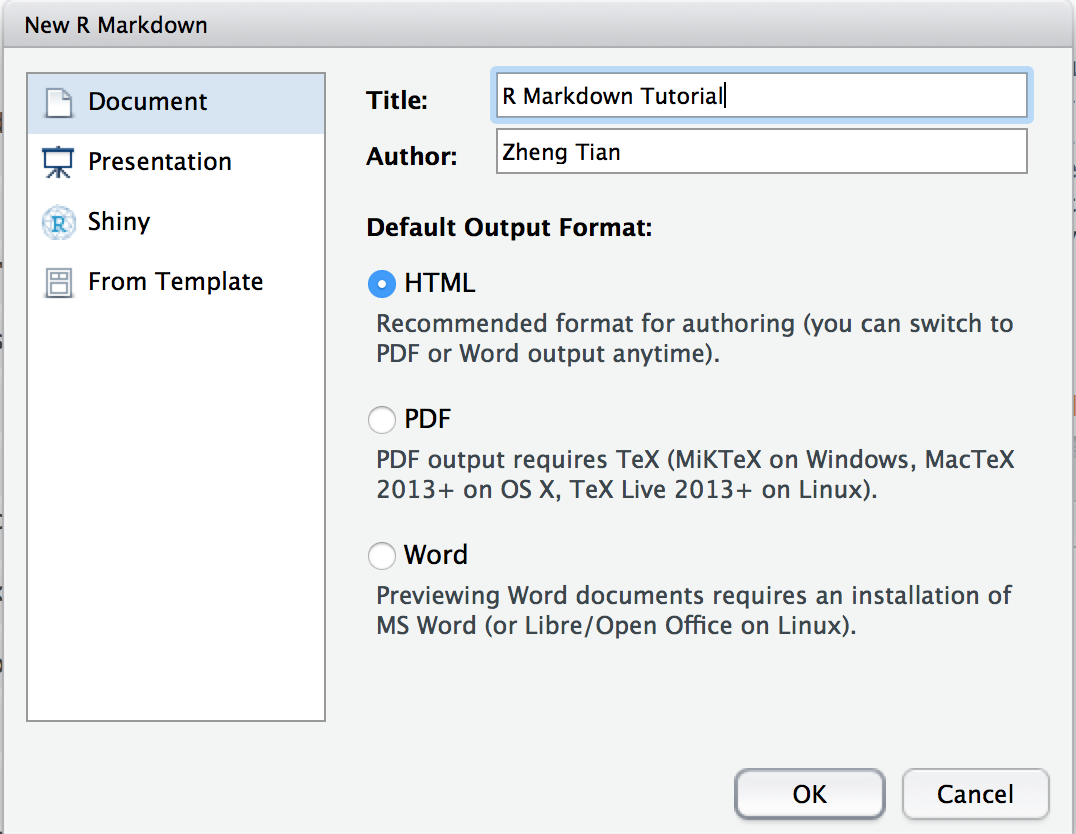
\includegraphics[width=.9\linewidth]{create_rmarkdown.png}
\end{center}}

\item A short R Markdown document is generated with some elements in it as
a template.
\end{enumerate}

\subsection*{How R Markdown works}
\label{sec:org0d8ac88}

The underlying mechanism of R Markdown is shown as follows

\begin{center}

\includegraphics[width=.9\linewidth]{rmarkdown_workflow.png}
\end{center}

\begin{itemize}
\item To generate an \texttt{HTML} document from a R Markdown file, click \texttt{Knit}
button in RStudio.
\item A built-in HTML browser will be invoked to have a preview of the
document.
\item You can also create a PDF file by click the little arrow beside
\texttt{Knit} button, and choose \texttt{Knit to PDF}.
\end{itemize}

\section{The Elements in a R Markdown File}
\label{sec:org5ad3711}

\subsection*{The Paragraph}
\label{sec:org6337edc}

A new paragraph is created by following one or more blank lines.

\subsection*{Headers and sections}
\label{sec:org963cf63}

The \texttt{\#} sign defines a top-level header and a section, \texttt{\#\#} defines a
level-two header and a subsection.

\begin{verbatim}
# Section
## A subsection
### A subsubsection
\end{verbatim}

\subsection*{Emphasis}
\label{sec:orgbf07f77}

Markdown uses \texttt{**bold**} to use the \textbf{bold} font and \texttt{*italic*} to use
the \emph{italic} font.

\subsection*{List}
\label{sec:org20d9470}

We can create a list as follows,

\begin{verbatim}
* Item 1
* Item 2
    + Item 2a
    + Item 2bn
\end{verbatim}

\begin{itemize}
\item Item 1
\item Item 2

\begin{itemize}
\item Item 2a
\item Item 2b
\end{itemize}
\end{itemize}

The list can also be numbered as follows,

\begin{verbatim}
1. Item 1
2. Item 2
3. Item 3
    + Item 3a
    + Item 3b
\end{verbatim}

\subsection*{Equations}
\label{sec:orgbb1b400}

R Markdown uses the \LaTeX{} command to create mathematical expressions.

For example, the linear regression equation in display mode is

\begin{verbatim}
\[Y_i = \beta_0 + \beta_1 X_i + u_i, \text{ for } i = 1, \ldots, n\]
\end{verbatim}

which generates
$$Y_i = \beta_0 + \beta_1 X_i + u_i, \text{ for } i = 1, \ldots, n$$

And the in-line mathematical expression is
\texttt{\$\textbackslash{}beta\_1 = \textbackslash{}frac\{\textbackslash{}Delta Y\}\{\textbackslash{}Delta X\}\$}, generating
\(\beta_1 = \frac{\Delta Y}{\Delta X}\).

\section{R Code Chunk}
\label{sec:org62e6c5d}

Most importantly, we can include R code along with the output in a R
Markdown file. You can quickly insert chunks like these into your file
with

\begin{itemize}
\item the keyboard shortcut \texttt{Ctrl + Alt + I} (OS X: \texttt{Cmd + Option + I})
\item the \texttt{Insert} button in the editor toolbar
\item or by typing the chunk delimiters \texttt{```\{r\}} and \texttt{```}.
\end{itemize}

The behaviors of the R code chunk can be controlled by adding options.

\begin{verbatim}
```{r, echo=TRUE, results='markup'}
summary(mtcars[, 1:3])
```
\end{verbatim}

\begin{verbatim}
     mpg             cyl             disp
Min.   :10.40   Min.   :4.000   Min.   : 71.1
1st Qu.:15.43   1st Qu.:4.000   1st Qu.:120.8
Median :19.20   Median :6.000   Median :196.3
Mean   :20.09   Mean   :6.188   Mean   :230.7
3rd Qu.:22.80   3rd Qu.:8.000   3rd Qu.:326.0
Max.   :33.90   Max.   :8.000   Max.   :472.0
\end{verbatim}

The options that are often used include \texttt{echo}, \texttt{results}, \texttt{include},
and \texttt{eval}, etc.

\begin{verbatim}
```{r, echo=TRUE, results='asis'}
library(knitr)
kable(mtcars[1:5, 1:3])
```
\end{verbatim}

\begin{verbatim}


|                  |  mpg| cyl| disp|
|:-----------------|----:|---:|----:|
|Mazda RX4         | 21.0|   6|  160|
|Mazda RX4 Wag     | 21.0|   6|  160|
|Datsun 710        | 22.8|   4|  108|
|Hornet 4 Drive    | 21.4|   6|  258|
|Hornet Sportabout | 18.7|   8|  360|
\end{verbatim}

We can also embed plots, for example:

\begin{verbatim}
```{r, echo=TRUE, fig.cap="A Scatterplot", fig.align='center', fig.pos="!h"}
  plot(mtcars$disp, mtcars$mpg,
       xlab = "displacement", ylab = "MPG")
```
\end{verbatim}

\begin{center}
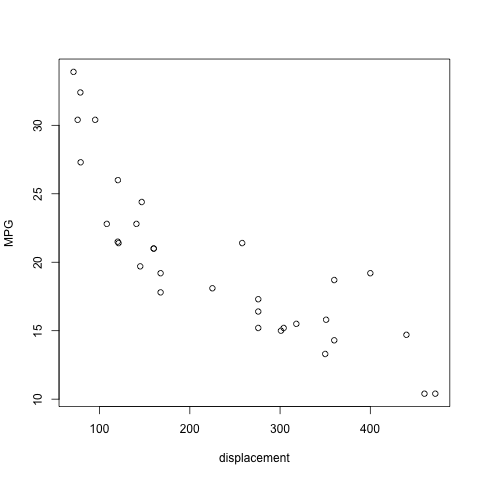
\includegraphics[width=.9\linewidth]{scatterplot.png}
\end{center}

Finally, we use the following reference card to quickly find the
relevant command in R Markdown,
\href{./rmarkdown\_cheatsheet.pdf}{rmarkdown\_cheatsheet.pdf}.
\end{document}